\documentclass{beamer}
\usepackage{hw}

\title{FlakeAutoFind}
\subtitle{Computer Vision Processing of Microscopy Photos}
\author{Charles Yang}
\date{7 January 2021}

\begin{document}
\frame{\titlepage}

\begin{frame}
	\frametitle{Problem Statement}
	\begin{itemize}
		\item<1-> From a microscopy image, determine where flakes are and infer their thickness. 
		\item<2-> Subproblems:
		\begin{itemize}
			\item<2-> The intensity of the flakes is very similar to the intensity of the background.
			\item<3-> The intensity of sensor noise is on the order of flake intensity.
			\item<4-> Determining the location of flakes and distinguishing them from other objects.
		\end{itemize}
	\end{itemize}
\end{frame}

\begin{frame}
	\frametitle{General Algorithm}
		Subproblems:
		\begin{itemize}
			\item<1-> The intensity of the flakes is very similar to the intensity of the background.
				\begin{itemize}
					\item<2-> Flattening and Contrast increase
				\end{itemize}
			\item<1-> The intensity of sensor noise is on the order of flake intensity.
				\begin{itemize}
					\item<3-> Blurring and Morphological transformations
				\end{itemize}
			\item<1-> Determining the location of flakes and distinguishing them from other objects.
				\begin{itemize}
					\item<4-> Edge Detection, Contouring, and Transmission Measurement (partial)
				\end{itemize}
		\end{itemize}
\end{frame}

\begin{frame}
	\frametitle{Flattening}
	\begin{itemize}
		\item<1-> Assuming elliptical symmetry, we define a distance metric 
			\[s^2 = (x-x_c)^2+r^2(y-y_c)^2\]
		\item<2-> Then, we claim that we can approximate the background as
			\[B(s) = \sum_n a_n s^{2n}\]
		\item<3-> Sampling multiple points, we then obtain a system of linear equations in \(a_n\)
			\[B_i = \sum_n a_n s_i^{2n}\]
	\end{itemize}
\end{frame}

\begin{frame}
	\frametitle{Flattening}
	\begin{itemize}
		\item<1-> Rewrite the previous as matrix equation
			\[B = SA\]
			with the vector of background values \(B_i\) being measured at points \(s_i\) to generate \(S_{ij} = s_i^{2(j-1)}\), with coefficients \(A_n = a_n\) 
		\item<2-> We strategically chose \(s_i\) to make computation easy:
			\[s_i^2 = (i+1)*s^2\]
			and suppress powers of \(s^2\) in the final matrix.
	\end{itemize}
\end{frame}

\begin{frame}
	\frametitle{Flattening}
	Performing row reduction on \(S\), we obtain a nice pattern:
	\[ [S'|I] = \left[ \begin{matrix} 1 & 1 & 1 & 1 & \cdots \\
			1 & 2 & 4 & 8 & \cdots \\
			1 & 3 & 9 & 27 & \cdots \\
			1 & 4 & 16 & 64 & \cdots\\
			\vdots & \vdots & \vdots & \vdots & \ddots
	\end{matrix} \,\middle\vert\, \begin{matrix}
			1 & 0 & 0 & 0 & \cdots \\
			0 & 1 & 0 & 0 & \cdots \\
			0 & 0 & 1 & 0 & \cdots \\
			0 & 0 & 0 & 1 & \cdots\\
			\vdots & \vdots & \vdots & \vdots & \ddots
	\end{matrix} \right]\]
	\[\dn\]
	\[ [T|C] = \left[ \begin{matrix}
			1 & 1 & 1 & 1 & \cdots\\
			0 & 1 & 3 & 7 & \cdots\\
			0 & 0 & 2 & 12 & \cdots\\
			0 & 0 & 0 & 6 & \cdots \\
			\vdots & \vdots & \vdots & \vdots & \ddots
	\end{matrix} \,\middle\vert\, \begin{matrix}
			1 & 0 & 0 & 0 &\cdots \\
			-1 & 1 & 0 & 0 &\cdots \\
			1 & -2 & 1 & 0 &\cdots \\
			-1 & 3 & -3 & 1 &\cdots \\
			\vdots & \vdots & \vdots & \vdots & \ddots
	\end{matrix} \right]\]
	This pattern was calculated and verified to hold until at least \(n=10\)
\end{frame}

\begin{frame}
	\frametitle{Flattening}
	\begin{itemize}
		\item<1-> Thus, we can obtain \(A\) by instead solving the equation
			\[CB = CSA\]
			using back substitution.
		\item<2-> Once \(A\) is determined, the baseline approximation can be computed recursively as
			\[f_0 = a_N\]
			\[f_n = s^2 f_{n-1}+a_{N-n}\]
			\[B_N(s) = f_N\]
		This baseline is then subtracted from the total image. After flattening, the contrast may be increased to make flakes more apparent,
	\end{itemize}
\end{frame}

\begin{frame}
	\frametitle{Flattening Results}
	Initial test: 2 fixed points
	\begin{center}
		\includegraphics[scale = 0.3]{image/magic2.png}
	\end{center}
\end{frame}

\begin{frame}
	\frametitle{Flattening Results}
	General: 1 Sample
	\begin{center}
		\includegraphics[scale = 0.25]{image/1samp.png}
	\end{center}
\end{frame}

\begin{frame}
	\frametitle{Flattening Results}
	General: 3 Sample
	\begin{center}
		\includegraphics[scale = 0.25]{image/3samp.png}
	\end{center}
\end{frame}

\begin{frame}
	\frametitle{Flattening Results}
	General: 5 Sample
	\begin{center}
		\includegraphics[scale = 0.25]{image/5samp.png}
	\end{center}
\end{frame}

\begin{frame}
	\frametitle{Blurring and Morphological Tranforms}
	\begin{itemize}
		\item<1->To reduce noise, first a gaussian blur was used to ``average out'' the noise in the initial image, before the process of flattening.
		\item<2->After flattening, the noise was further removed using a combination of the morphological transformations Open, Close, Erode, Dilate included in the OpenCV API.
		\begin{itemize}
			\item<3-> Erosion returns 1 only if all pixels in the kernel are 1
			\item<4-> Dilation returns 1 if any pixel in the kernel is 1
			\item<5-> Opening and Closure are both compositions of the Erosion and Dilation
		\end{itemize}
		\item<6-> The morphological transforms were determined by trial and error, adjusting the order of transformation and size of the kernel.
	\end{itemize}
\end{frame}

\begin{frame}
	\frametitle{Denoising Results}
	\begin{center}
		\includegraphics[scale = 0.3]{image/morph1.png}
	\end{center}
\end{frame}

\begin{frame}
	\frametitle{Denoising Results}
	\begin{center}
		\includegraphics[scale = 0.3]{image/morph2.png}
	\end{center}
\end{frame}

\begin{frame}
	\frametitle{Edge Detection, Contouring, and Transmission Measurement (partial)}
	\begin{itemize}
		\item<1-> Edge detection is can be done using a gradient method, such as Sobel Derivatives and the Laplacian, to detect where the intensity of an image changes quickly---an ``edge''
		\item<2-> After the edges are detected, they are thresholded to only allow for stronger edges to remain. The \emph{contour} method of OpenCV then generates sets of points on isolines---contours---as the sets of boundaries
		\item<3-> The flakes can be inferred to be regions contained within closed boundaries.
		\item<4-> The flakes can be filtered from noise and other objects by measuring the transmission relative to the approximated baseline.
		\item<5-> While I have proposed these methods, I haven't been able to test them as extensively.
	\end{itemize}
\end{frame}

\begin{frame}
	\frametitle{Flake Determination Results}
	Morphology, Contrast bump, Sobel Derivative
	\begin{center}
		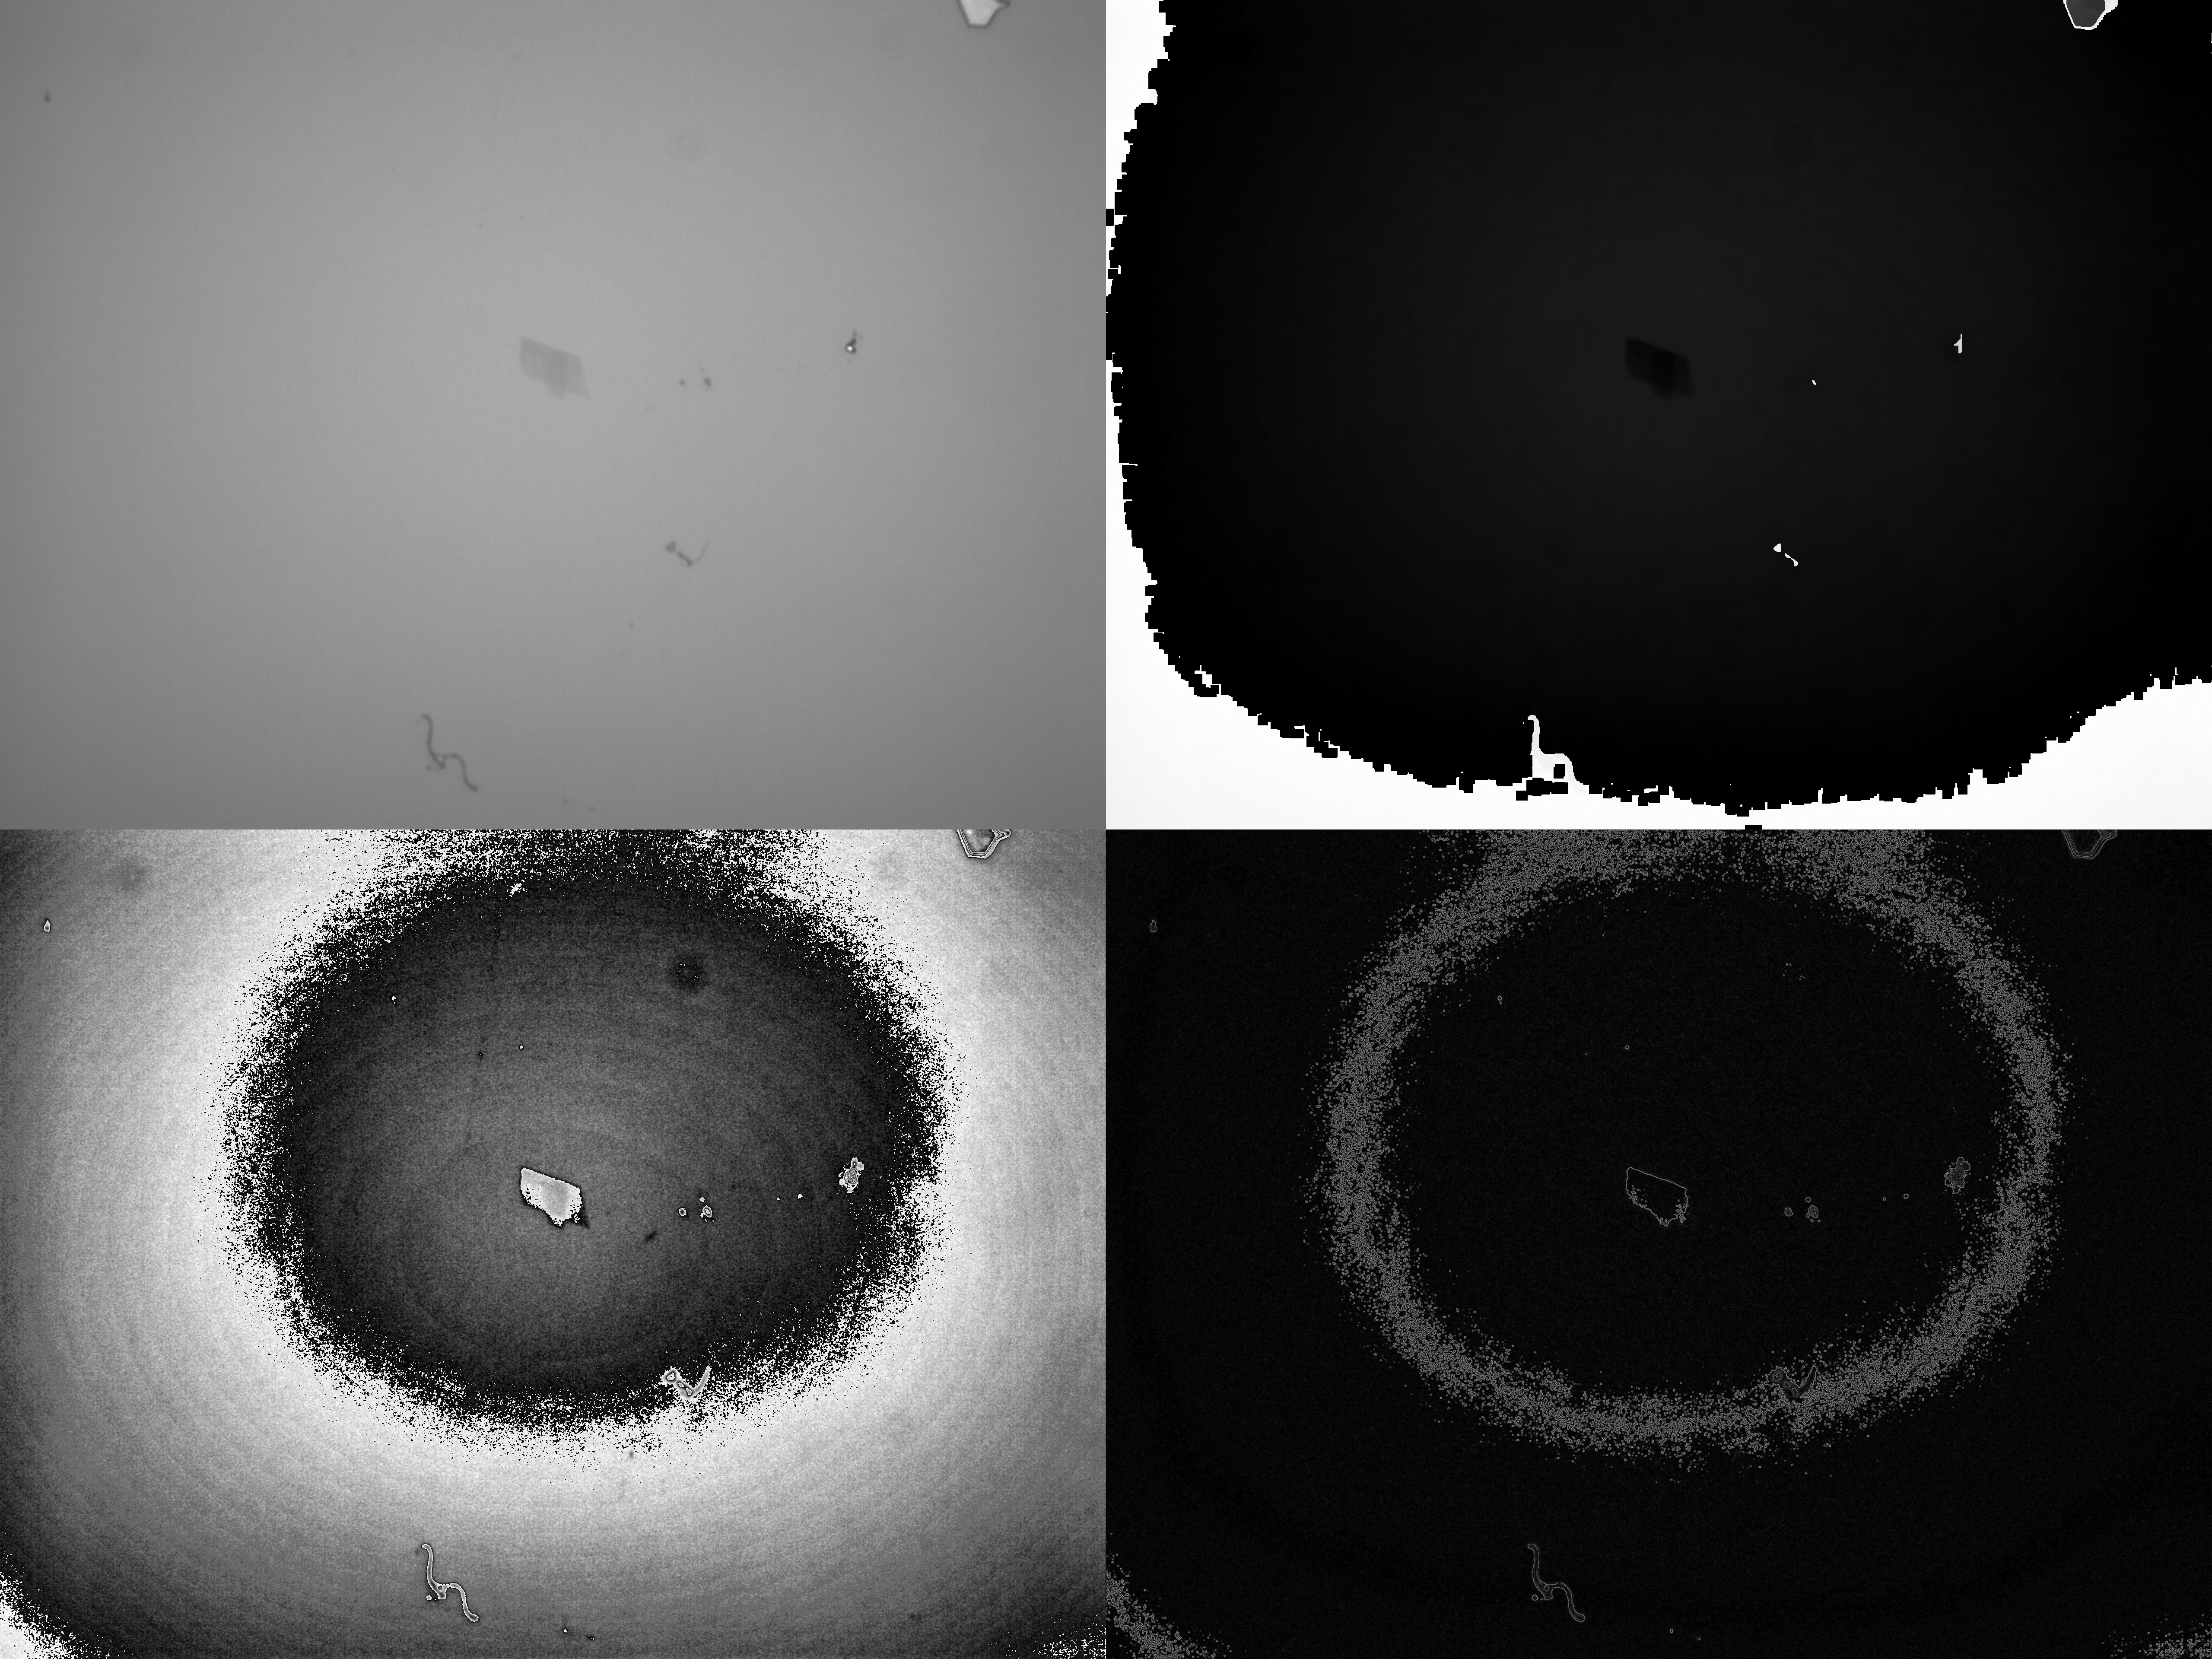
\includegraphics[scale=0.05]{image/closecontrastsobel.png}
	\end{center}
\end{frame}

\begin{frame}
	\frametitle{Flake Determination Results}
	Morphology, Contrast bump, Sobel Derivative
	\begin{center}
		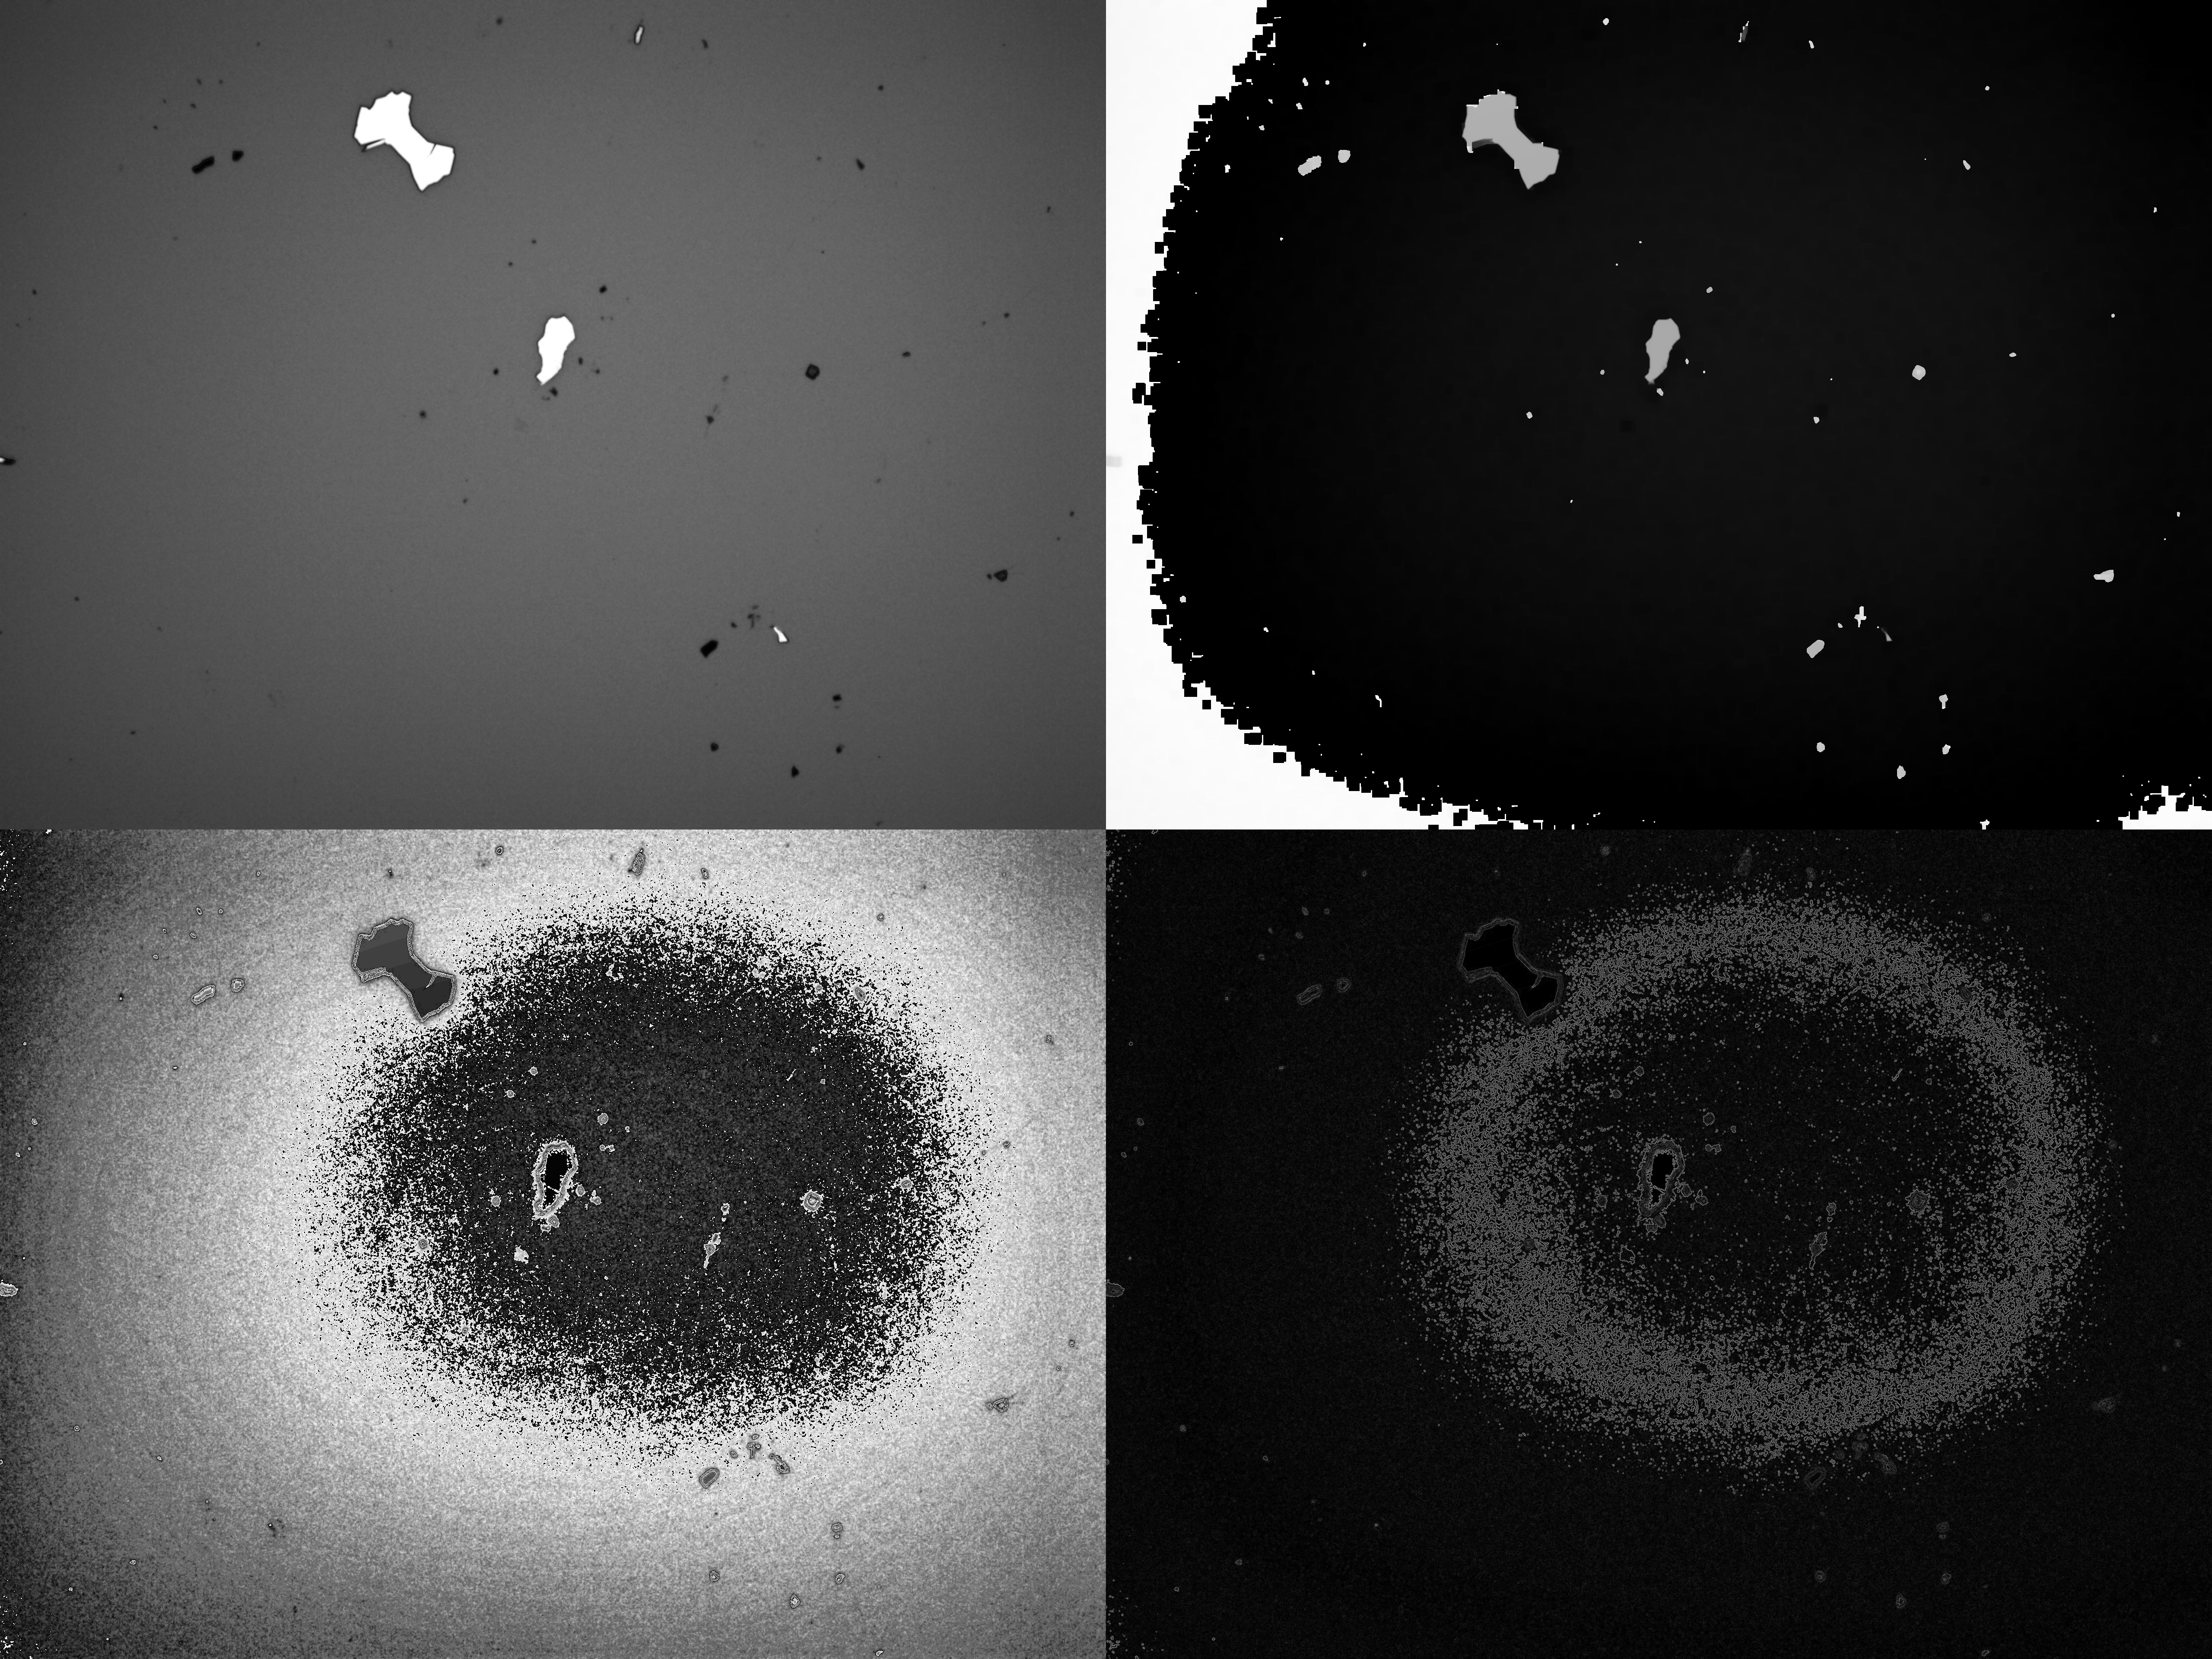
\includegraphics[scale=0.05]{image/closecontrastsobel2-4-20.png}
	\end{center}
\end{frame}

\begin{frame}
	\frametitle{Flake Determination Results}
	Morphology, Contrast bump, Laplacian
	\begin{center}
		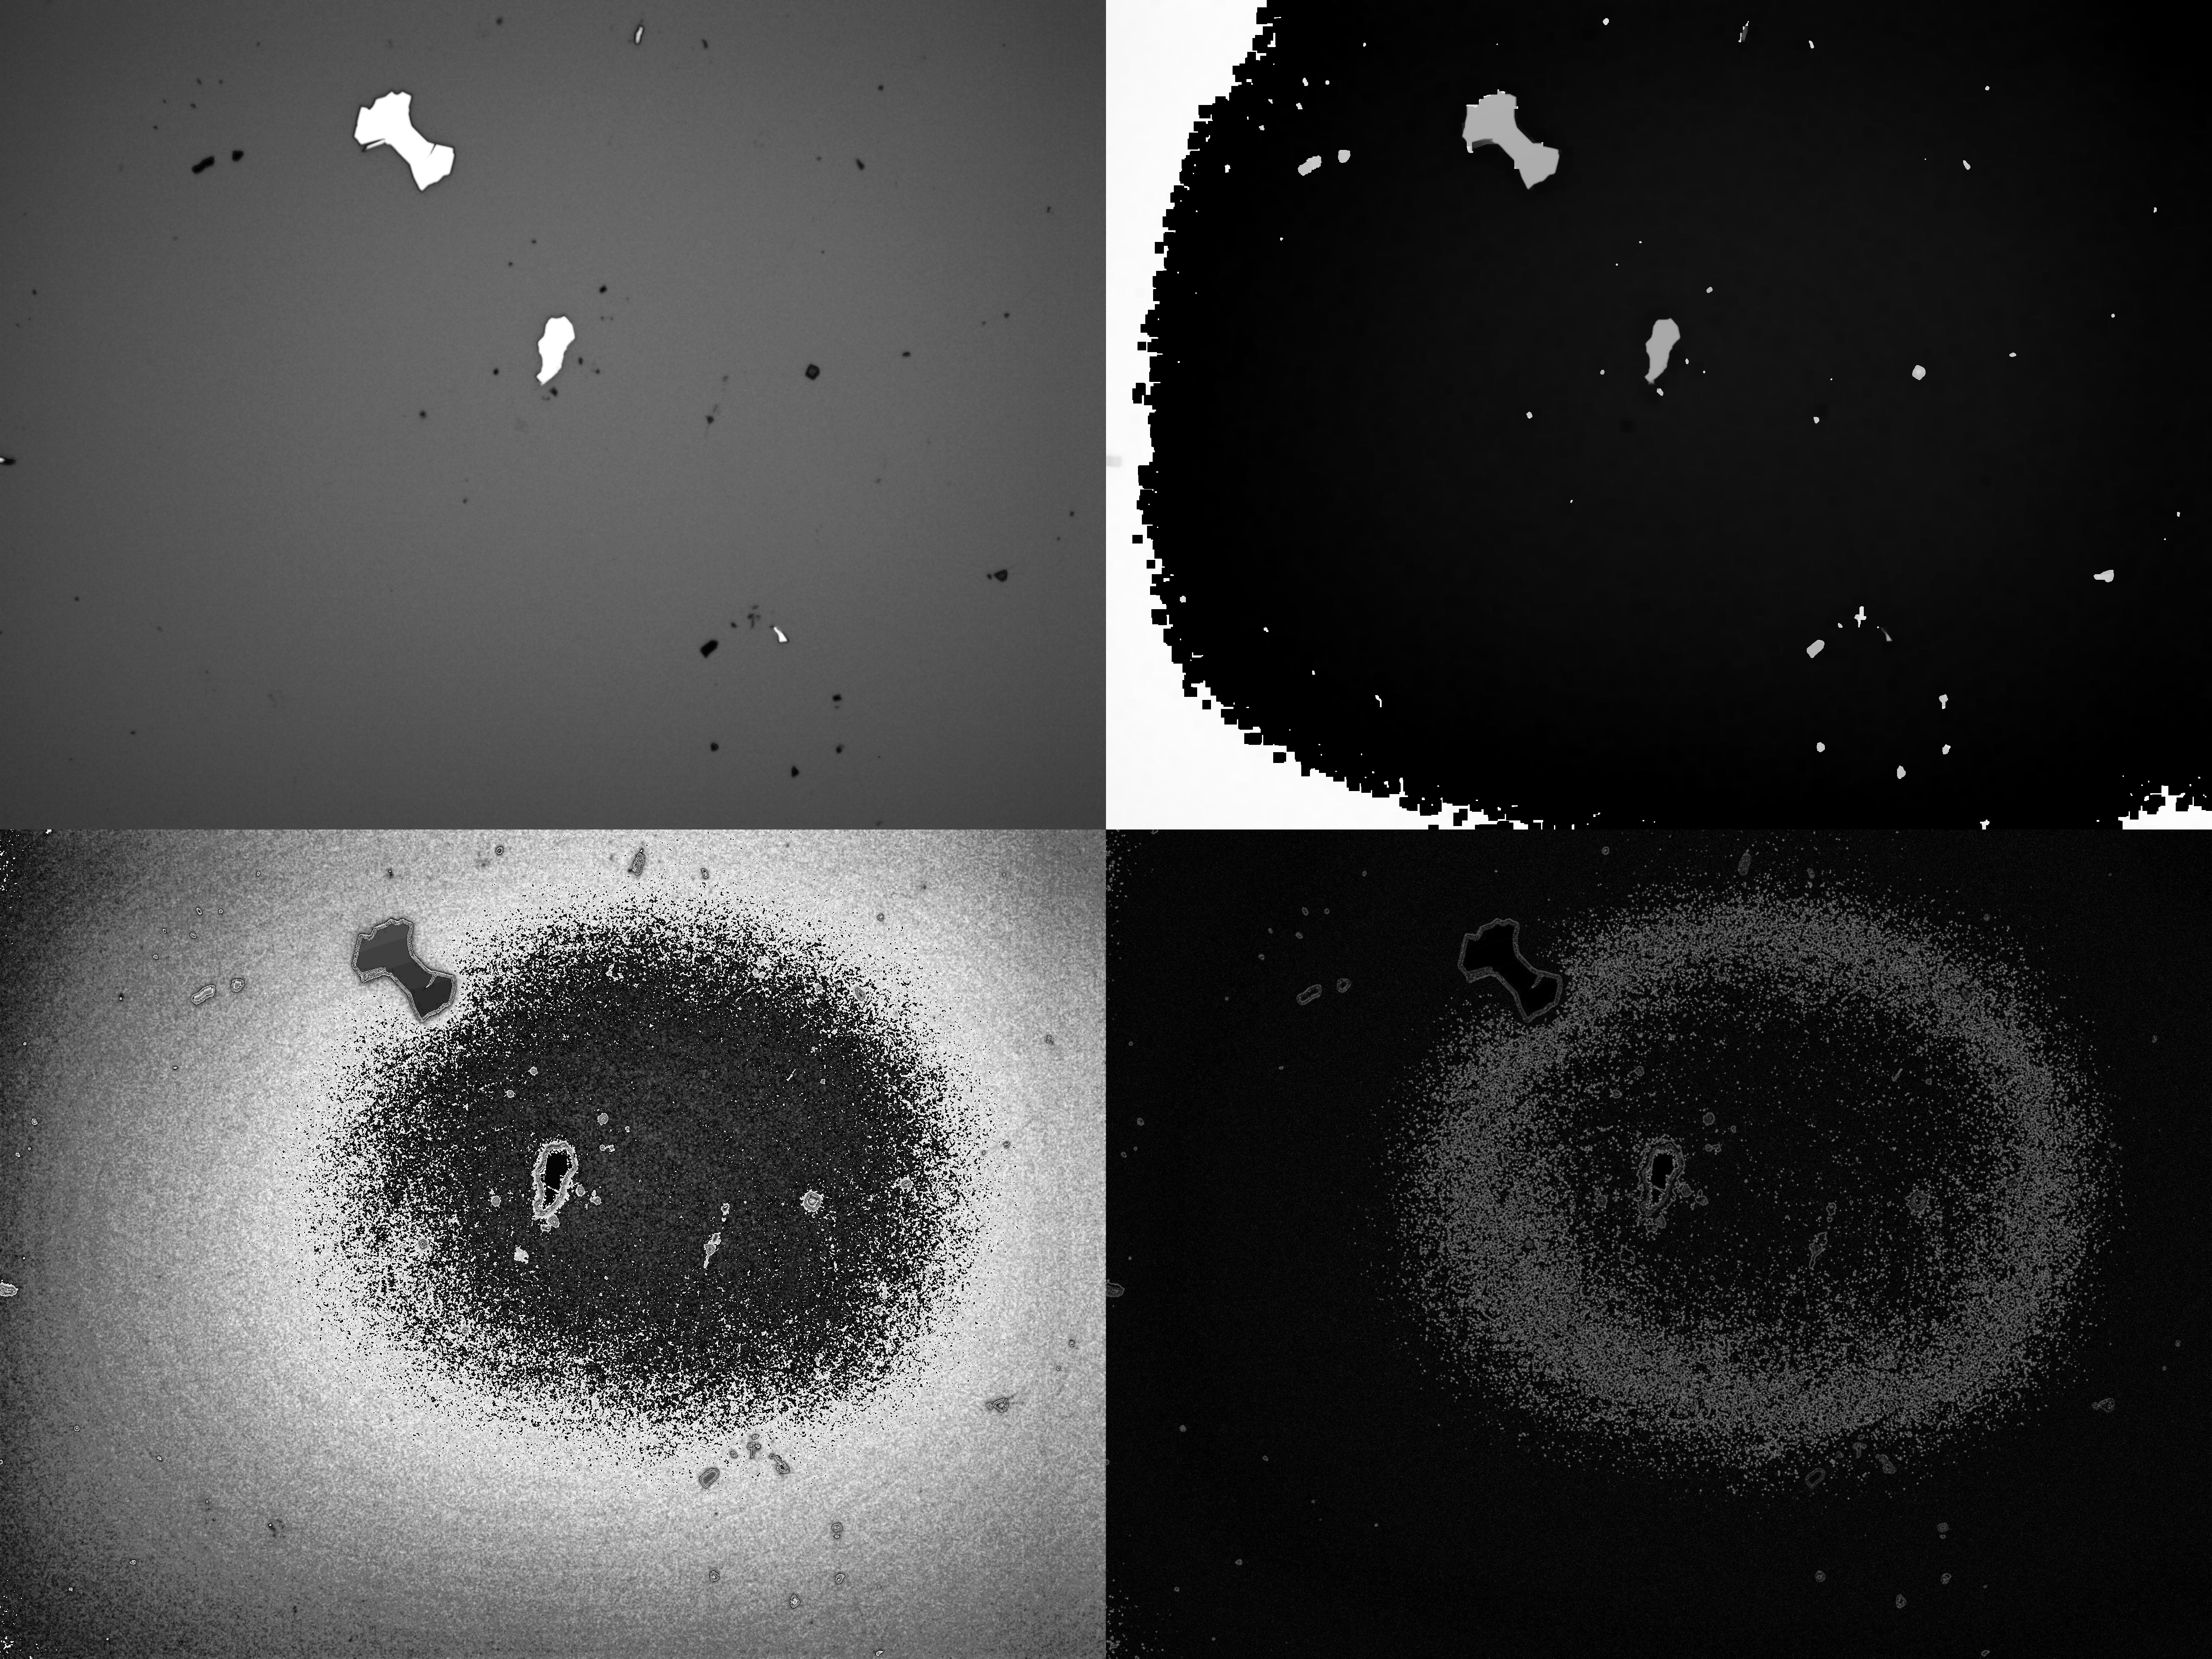
\includegraphics[scale=0.05]{image/closecontrastlaplacian2-4-20.png}
	\end{center}
\end{frame}

\begin{frame}
	\frametitle{Flake Determination Results}
	Contours
	\begin{center}
		\includegraphics[scale=0.13]{image/contourbefore.png}
		\includegraphics[scale=0.13]{image/contour.png}
	\end{center}
\end{frame}

\begin{frame}
	\frametitle{Issues and Directions for Future Work}
	\begin{itemize}
		\item<1-> Background isn't perfectly centred or uniform as assumed.
		\item<2-> Very low signal to noise ratio---Image stacking?
		\item<3-> Many of the transformations need specified kernel sizes---introduction of ``magic numbers''
		\item<4-> The latter half of the program could not be implemented due to issues with the flattening algorithm.
		\item<5-> Alternative colour spaces may be better suited for analysis than the default BGR colourspace.
	\end{itemize}
	
\end{frame}

\begin{frame}
	\frametitle{Code}
	https://github.com/daedalus1235/FlakeAutoFind.git (private repo)

	Written in C++ using OpenCV, compiled with CMake and g++.
\end{frame}

\end{document}
